\documentclass[11pt,a4paper]{report}

% ---------------------------------------------------------------------------
% Packages
% ---------------------------------------------------------------------------
\usepackage[T1]{fontenc}
\usepackage[utf8]{inputenc}
\usepackage{lmodern}
\usepackage{microtype}
\usepackage[margin=2.5cm]{geometry}
\usepackage{setspace}
\usepackage{graphicx}
\usepackage{booktabs}
\usepackage{longtable}
\usepackage{array}
\usepackage{tabularx}
\usepackage{xcolor}
\usepackage{amsmath}
\usepackage{enumitem}
\usepackage{float}
\usepackage{caption}
\usepackage{listings}
\usepackage{algorithm}
\usepackage{algpseudocode}
\usepackage{pdflscape}
\usepackage{tikz}
\usetikzlibrary{positioning,arrows.meta,shapes.multipart,fit,calc}
\usepackage{pgfplots}
\pgfplotsset{compat=1.17}
\usepackage[numbers,sort&compress]{natbib}
\usepackage{url}
\usepackage[hidelinks]{hyperref}

\onehalfspacing
\setlength{\emergencystretch}{3em}
\setlist{itemsep=2pt,topsep=4pt}

% ---------------------------------------------------------------------------
% Colours and listings
% ---------------------------------------------------------------------------
\definecolor{navy}{HTML}{131B2E}
\definecolor{teal}{HTML}{0B7A6F}
\definecolor{crit}{HTML}{C8353A}
\definecolor{high}{HTML}{B8730F}
\definecolor{med}{HTML}{92650A}
\definecolor{healthy}{HTML}{0F9488}
\definecolor{codebg}{HTML}{F4F6FB}

\lstdefinestyle{code}{
  basicstyle=\ttfamily\footnotesize,
  backgroundcolor=\color{codebg},
  frame=single, rulecolor=\color{gray!40},
  keywordstyle=\color{navy}\bfseries,
  commentstyle=\color{teal}\itshape,
  stringstyle=\color{crit},
  breaklines=true, columns=fullflexible,
  showstringspaces=false, tabsize=4,
  xleftmargin=4pt, xrightmargin=4pt, aboveskip=8pt, belowskip=8pt
}
\lstdefinelanguage{MySQL}[]{SQL}{
  morekeywords={WITH,OVER,PARTITION,ROW_NUMBER,RETURNS,DETERMINISTIC,TRIGGER,
    AFTER,EACH,ROW,BEGIN,END,DECLARE,IF,THEN,ELSE,ELSEIF,PROCEDURE,FUNCTION,
    CALL,REPLACE,VIEW,LIMIT,INTERVAL,DAY,WEEK,MONTH,LEFT,DELIMITER,NEW,
    DUPLICATE,KEY,CASCADE,ENUM,ENGINE,AUTO_INCREMENT,FIELD,DATEDIFF,
    TIMESTAMPDIFF,NULLIF,COALESCE},
  sensitive=false
}
\lstset{style=code}

\captionsetup{font=small,labelfont=bf}

% The bibliography chapter is titled "References"
\renewcommand{\bibname}{References}

% Small helper for risk labels in tables
\newcommand{\risk}[1]{\textsf{\small #1}}

% ---------------------------------------------------------------------------
\begin{document}

% ---------------------------------------------------------------------------
% Title page
% ---------------------------------------------------------------------------
\begin{titlepage}
\centering
\vspace*{1cm}
{\large Amrita Vishwa Vidyapeetham\par}
{\normalsize Department of Artificial Intelligence\par}
\vspace{2.2cm}
{\Large\bfseries Database Management Systems --- Course Project Report\par}
\vspace{1.2cm}
{\rule{\linewidth}{0.6pt}\par\vspace{0.4cm}}
{\Huge\bfseries Bus Factor Tracker\par}
\vspace{0.4cm}
{\Large Estimating Open-Source Maintainer Burnout and Bus Factor Risk from Real GitHub Data\par}
\vspace{0.4cm}
{\rule{\linewidth}{0.6pt}\par}
\vspace{2cm}
{\large Submitted by\par}
\vspace{0.4cm}
{\large
\begin{tabular}{l l}
Dhakshin & CB.SC.U4AIE24313 \\
Rohith Ravi & CB.SC.U4AIE24350 \\
Sanjay Kumar S & CB.SC.U4AIE24354 \\
Akhilan & CB.SC.U4AIE24362 \\
\end{tabular}\par}
\vfill
{\large Semester V \quad\textbullet\quad October 2026\par}
\end{titlepage}

% ---------------------------------------------------------------------------
\begin{abstract}
\noindent
Open-source software forms the base layer of almost every modern application,
yet much of it is maintained by a handful of volunteers. When such a maintainer
burns out or leaves, every project that depends on their work is exposed, often
with no warning. The \emph{bus factor} of a project, the number of people who
would have to disappear before it stalls, is a simple measure of this risk.

This report presents the \textbf{Bus Factor Tracker}, a database-centred system
that estimates bus factor and maintainer-burnout risk for real GitHub
repositories from public data only. A Python sync engine pulls repository
metadata, per-contributor weekly commit counts, issues, pull requests and
releases from the GitHub REST API into a MySQL~8.0 database of ten relations in
Boyce--Codd normal form, writing each repository inside a single ACID
transaction. Automation bots are identified and excluded, and the bus factor is
computed in SQL with common table expressions and window functions over the
last twelve months of commits, falling back to the all-time value for
repositories with too little recent work. Burnout signals (no recent commits,
falling commit activity, an inactive key contributor and slow issue responses)
raise a base risk level derived from the bus factor. Because the weekly data
goes back years, the first sync rebuilds a year of monthly snapshots, so trends
are available immediately. A view, a stored function, a stored procedure and a
trigger expose the latest risk, detect declining repositories and record every
risk increase, comparing only snapshots produced by the same version of the
scoring method. A FastAPI service and a React dashboard present the results
with a plain-English explanation of each score.

Applied to 42 widely used repositories (17,306 contributors, 273,603
contributor-weeks of commits, 16,490 pull requests), the system found that 21
repositories (50\%) depend on a single person for at least half of their
recent commits. The rebuilt history contains 16 risk increases, all recorded by
the trigger, including a fall in the bus factor of \texttt{httpx} from 5 to~1
within six months. Excluding bots changed the picture for large projects:
Kubernetes' all-time bus factor rose from 18 to 44 once its CI robot was
removed. All read endpoints of the API respond in about 10\,ms or less.

\vspace{0.6em}
\noindent\textbf{Keywords:} bus factor, truck factor, open-source sustainability,
maintainer burnout, relational database, MySQL, window functions, triggers,
time-series snapshots, GitHub REST API.
\end{abstract}

\tableofcontents
\listoffigures
\listoftables

% ===========================================================================
\chapter{Introduction}
% ===========================================================================

\section{Background}

Open-source libraries are reused at enormous scale: a single web application
can pull in hundreds of transitive dependencies, each maintained by people the
application's developers have never met. Studies of the open-source ecosystem
describe this as critical public infrastructure that is largely maintained
without pay~\cite{eghbal2016roads,eghbal2020working}. The consequences of a
single maintainer's decision became widely visible in March 2016, when the
removal of the eleven-line \texttt{left-pad} package from the npm registry
broke the builds of thousands of downstream projects~\cite{npm2016leftpad}.

Less dramatic versions of the same failure happen continually. Maintainers
lose interest, change jobs or simply burn out, and projects that looked healthy
from the outside stop receiving fixes. Research on failed open-source projects
lists lack of maintainer time and interest among the most common reasons a
project is abandoned~\cite{coelho2017fail}, and toxic or demanding interactions
with users are a documented source of maintainer stress~\cite{raman2020stress}.

\section{The bus factor}

The \emph{bus factor} (also called the \emph{truck factor}) of a software
project is the minimum number of developers who would have to leave the project
(``be hit by a bus'') before it can no longer be maintained. A bus factor of~1
means that a single person holds knowledge or responsibility the project cannot
function without. Several algorithms have been proposed to estimate it from
version-control history, including file-authorship approaches
\cite{avelino2016truck} and commit-based approaches applied directly to Git
repositories~\cite{cosentino2015bus}. Practitioners report that the metric is
useful but that raw estimates need context to be acted on~\cite{jabrayilzade2022bus}.

\section{Problem statement}

Developers choosing a dependency, and organisations funding open-source work,
have no simple way to see which projects are one person away from
abandonment. Existing tools either show raw activity graphs for a single
repository, focus on security practices, or require a heavyweight analytics
platform (Section~\ref{sec:related}). The problem addressed in this project is:

\begin{quote}
\itshape
Design and build a database-backed system that estimates the bus factor and
maintainer-burnout risk of real GitHub repositories from public data,
explains each estimate, and tracks how the risk changes over time.
\end{quote}

\section{Objectives}

\begin{enumerate}
  \item Collect real repository, contributor, issue, pull-request and release
        data from the GitHub REST API --- no simulated data.
  \item Design a normalised relational schema (BCNF) with full referential
        integrity, suitable for both current-state queries and time-series
        history.
  \item Compute the bus factor, median issue-response time and burnout signals
        inside the database using SQL (CTEs and window functions).
  \item Use DBMS features where they fit the problem: transactions for
        consistent syncs, a view, a stored function, a stored procedure and a
        trigger.
  \item Combine the measurements into an explainable risk level per
        repository, and record every increase in risk.
  \item Present the results through a REST API and an interactive web
        dashboard.
\end{enumerate}

\section{Scope}

The system tracks a configurable list of public GitHub repositories (42 in the
evaluation, chosen to mix large, well-staffed projects with small
single-maintainer utilities and one archived project). It relies on the data
GitHub exposes through its public API with a personal access token. It does not
analyse source code, mailing lists or chat channels, and it does not attempt
per-file authorship analysis.

\section{Related work}
\label{sec:related}

\paragraph{Truck-factor research.} Avelino et al.~\cite{avelino2016truck}
estimate truck factors from file authorship (degree-of-authorship) and
validate the estimates with developers of popular GitHub projects. Cosentino
et al.~\cite{cosentino2015bus} compute bus-factor indicators for Git
repositories. Jabrayilzade et al.~\cite{jabrayilzade2022bus} study how the bus
factor is used in industry. These works analyse repositories at a point in
time; they do not maintain a continuously updated history or alert on change.

\paragraph{Community-health tooling.} The CHAOSS project~\cite{chaoss} defines a
broad catalogue of open-source community-health metrics and provides
analytics platforms to compute them. The OpenSSF Scorecard~\cite{scorecard}
assesses security-related practices of a repository, including whether it has
been recently active. GitHub's own repository Insights pages show activity
graphs for one repository at a time.

\paragraph{This project.} The Bus Factor Tracker sits between these: it is a
lightweight, single-purpose system that (i) combines commit concentration with
burnout signals into one explainable risk level, (ii) ranks many repositories
side by side, and (iii) keeps an append-only history so that declines and risk
increases are detected inside the database itself.

\section{Organisation of the report}

Chapter~\ref{ch:method} describes the system architecture, data collection,
database design, SQL techniques and risk-scoring method.
Chapter~\ref{ch:results} presents the results on 42 real repositories and
discusses them, including performance, validation cases and limitations.
Chapter~\ref{ch:conclusion} concludes and outlines future work.

% ===========================================================================
\chapter{Methodology}
\label{ch:method}
% ===========================================================================

\section{System architecture}

The system is split into four modules connected by the database
(Figure~\ref{fig:arch}). Collecting data is slow (tens of seconds of API calls
per repository) while reading results must be fast, so the two are deliberately
separated: the sync engine writes, and the API almost only reads.

\begin{figure}[H]
\centering
\resizebox{\textwidth}{!}{%
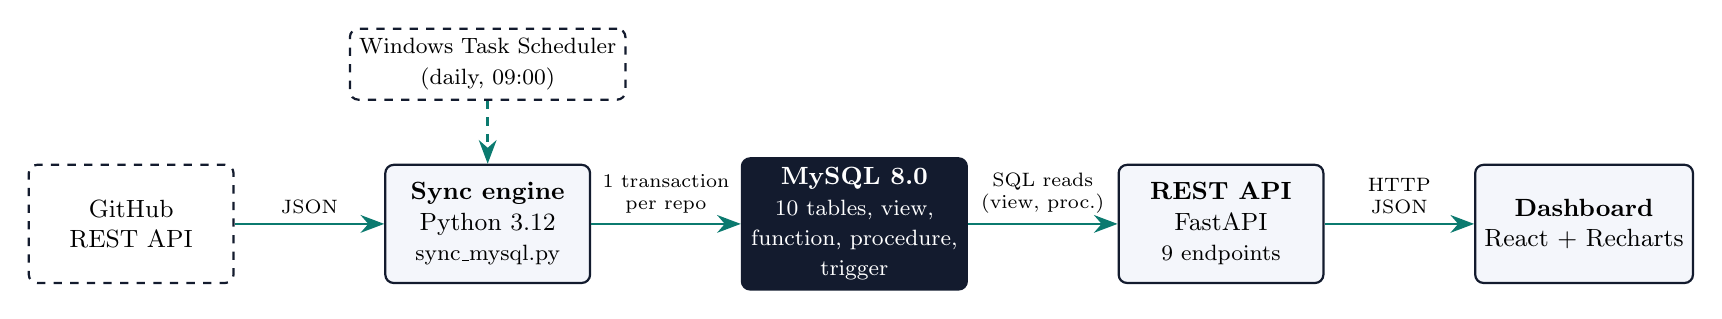
\begin{tikzpicture}[
  box/.style={draw=navy, line width=0.8pt, rounded corners=3pt, fill=codebg,
              minimum height=1.5cm, minimum width=2.6cm, align=center, font=\small},
  ext/.style={box, fill=white, dashed},
  arr/.style={-{Stealth[length=3mm]}, line width=0.9pt, draw=teal}
]
\node[ext] (gh) {GitHub\\REST API};
\node[box, right=1.9cm of gh] (sync) {\textbf{Sync engine}\\Python 3.12\\\footnotesize sync\_mysql.py};
\node[box, right=1.9cm of sync, fill=navy, text=white] (db) {\textbf{MySQL 8.0}\\\footnotesize 10 tables, view,\\\footnotesize function, procedure,\\\footnotesize trigger};
\node[box, right=1.9cm of db] (api) {\textbf{REST API}\\FastAPI\\\footnotesize 9 endpoints};
\node[box, right=1.9cm of api] (ui) {\textbf{Dashboard}\\React + Recharts};
\node[ext, above=0.8cm of sync, minimum height=0.9cm] (sched) {\footnotesize Windows Task Scheduler\\\footnotesize (daily, 09:00)};
\draw[arr] (gh) -- node[above, font=\scriptsize, align=center]{JSON} (sync);
\draw[arr] (sync) -- node[above, font=\scriptsize, align=center]{1 transaction\\per repo} (db);
\draw[arr] (db) -- node[above, font=\scriptsize, align=center]{SQL reads\\(view, proc.)} (api);
\draw[arr] (api) -- node[above, font=\scriptsize, align=center]{HTTP\\JSON} (ui);
\draw[arr, dashed] (sched) -- (sync);
\end{tikzpicture}}
\caption{System architecture and data flow.}
\label{fig:arch}
\end{figure}

\section{Data collection}

The sync engine (\texttt{scripts/sync\_mysql.py}) reads the list of tracked
repositories from \texttt{repos.txt} and, for each repository, calls the GitHub
REST API endpoints in Table~\ref{tab:endpoints}~\cite{github_rest}.

\begin{table}[H]
\centering
\caption{GitHub REST API endpoints used per repository.}
\label{tab:endpoints}
\small
\begin{tabularx}{\textwidth}{>{\ttfamily}l X}
\toprule
\textrm{\textbf{Endpoint}} & \textbf{Data obtained} \\
\midrule
/repos/\{o\}/\{r\} & Language, stars, forks, creation date, archived flag \\
/repos/\{o\}/\{r\}/stats/contributors & For each of the top 100 contributors: account type and commits, additions and deletions per week since the repository began \\
/repos/\{o\}/\{r\}/stats/commit\_activity & Total commits per week for the last 52 weeks \\
/repos/\{o\}/\{r\}/issues & Issues (state, opened/closed time, author); pull requests filtered out \\
/repos/\{o\}/\{r\}/issues/\{n\}/comments & Comments on an issue, giving the first-response time \\
/repos/\{o\}/\{r\}/pulls & Pull requests (state, opened/merged time, author) \\
/repos/\{o\}/\{r\}/releases & Releases (tag, publish time, author) \\
\bottomrule
\end{tabularx}
\end{table}

Several design choices keep the sync within GitHub's limit of 5,000
authenticated requests per hour and make it robust:

\begin{itemize}
  \item \textbf{Pre-aggregated statistics.} Contributor and weekly-activity
        statistics come from GitHub's \texttt{stats} endpoints, one call each,
        instead of one call per commit.
  \item \textbf{Incremental sync.} The repository's \texttt{last\_synced\_at}
        timestamp is read before each sync; issues are requested with GitHub's
        \texttt{since} parameter, and pull-request and release pagination stops
        as soon as it reaches items older than the last sync.
  \item \textbf{Capped work.} Pagination is capped at three pages, and the
        first-response lookup is limited to the 30 most recently updated
        issues with comments; those lookups run concurrently (10 threads).
  \item \textbf{Lazy statistics.} GitHub computes \texttt{stats} endpoints in the
        background and answers \texttt{202 Accepted} until they are ready. The
        engine retries with capped exponential back-off (2, 4, 8, 10, 10\,s).
        If \texttt{commit\_activity} never becomes ready, weekly totals are
        derived from the per-contributor weekly counts instead.
  \item \textbf{Network resilience.} Dropped connections, truncated responses
        and time-outs are retried up to three times per request.
  \item \textbf{No network I/O inside a transaction.} All API calls for a
        repository complete before its database transaction begins, so slow
        responses never hold locks.
\end{itemize}

\paragraph{Bot detection.} Many projects run automation accounts that commit,
merge or comment on everyone's behalf. GitHub marks GitHub Apps with the account
type \texttt{Bot} (e.g.\ \nolinkurl{dependabot[bot]}), but many CI bots are
ordinary user accounts (\nolinkurl{k8s-ci-robot}, \nolinkurl{pytorchmergebot},
\nolinkurl{tensorflower-gardener}). An account is therefore treated as a bot if
its type is \texttt{Bot} or its login ends in \texttt{[bot]}, \texttt{bot} or
\texttt{-gardener}. Checked against all 17,306 contributors in the data set,
the rule flags 52 accounts; the few that may be people with ``bot''-like names
have 60 commits or fewer, too few to affect any bus factor. Bots are kept in the
database (flag \texttt{contributor.is\_bot}) but excluded from every
calculation.

\paragraph{First response to an issue.} The first-response time is the time of
the first comment by someone other than the issue's author who is not a bot.
Taking simply the first comment would measure bots: on Go, Kubernetes and
PyTorch, a bot comments on every new issue within seconds.

A Windows Task Scheduler job runs the sync daily, so that each repository gains
one snapshot per day.

\section{Database design}

\subsection{Entity--relationship model}

The conceptual model (Figure~\ref{fig:er}) follows Chen's entity--relationship
approach~\cite{chen1976er}. \textsc{Repository} and \textsc{Contributor} are the
two strong entities. Their many-to-many relationship carries its own
attributes (commit counts and first/last commit dates), so it is modelled as
the associative entity \textsc{Repo\_Contributor}. Each repository--contributor
pair is further broken down by week in \textsc{Contributor\_Weekly\_Commits},
a weak entity identified by the pair and the week; it is what allows the bus
factor to be computed for any time window and as of any past date.
\textsc{Weekly\_Activity} is a weak entity identified by its repository and
week. Snapshots and alerts form an append-only history.

\begin{landscape}
\begin{figure}[p]
\centering
\resizebox{\linewidth}{!}{%
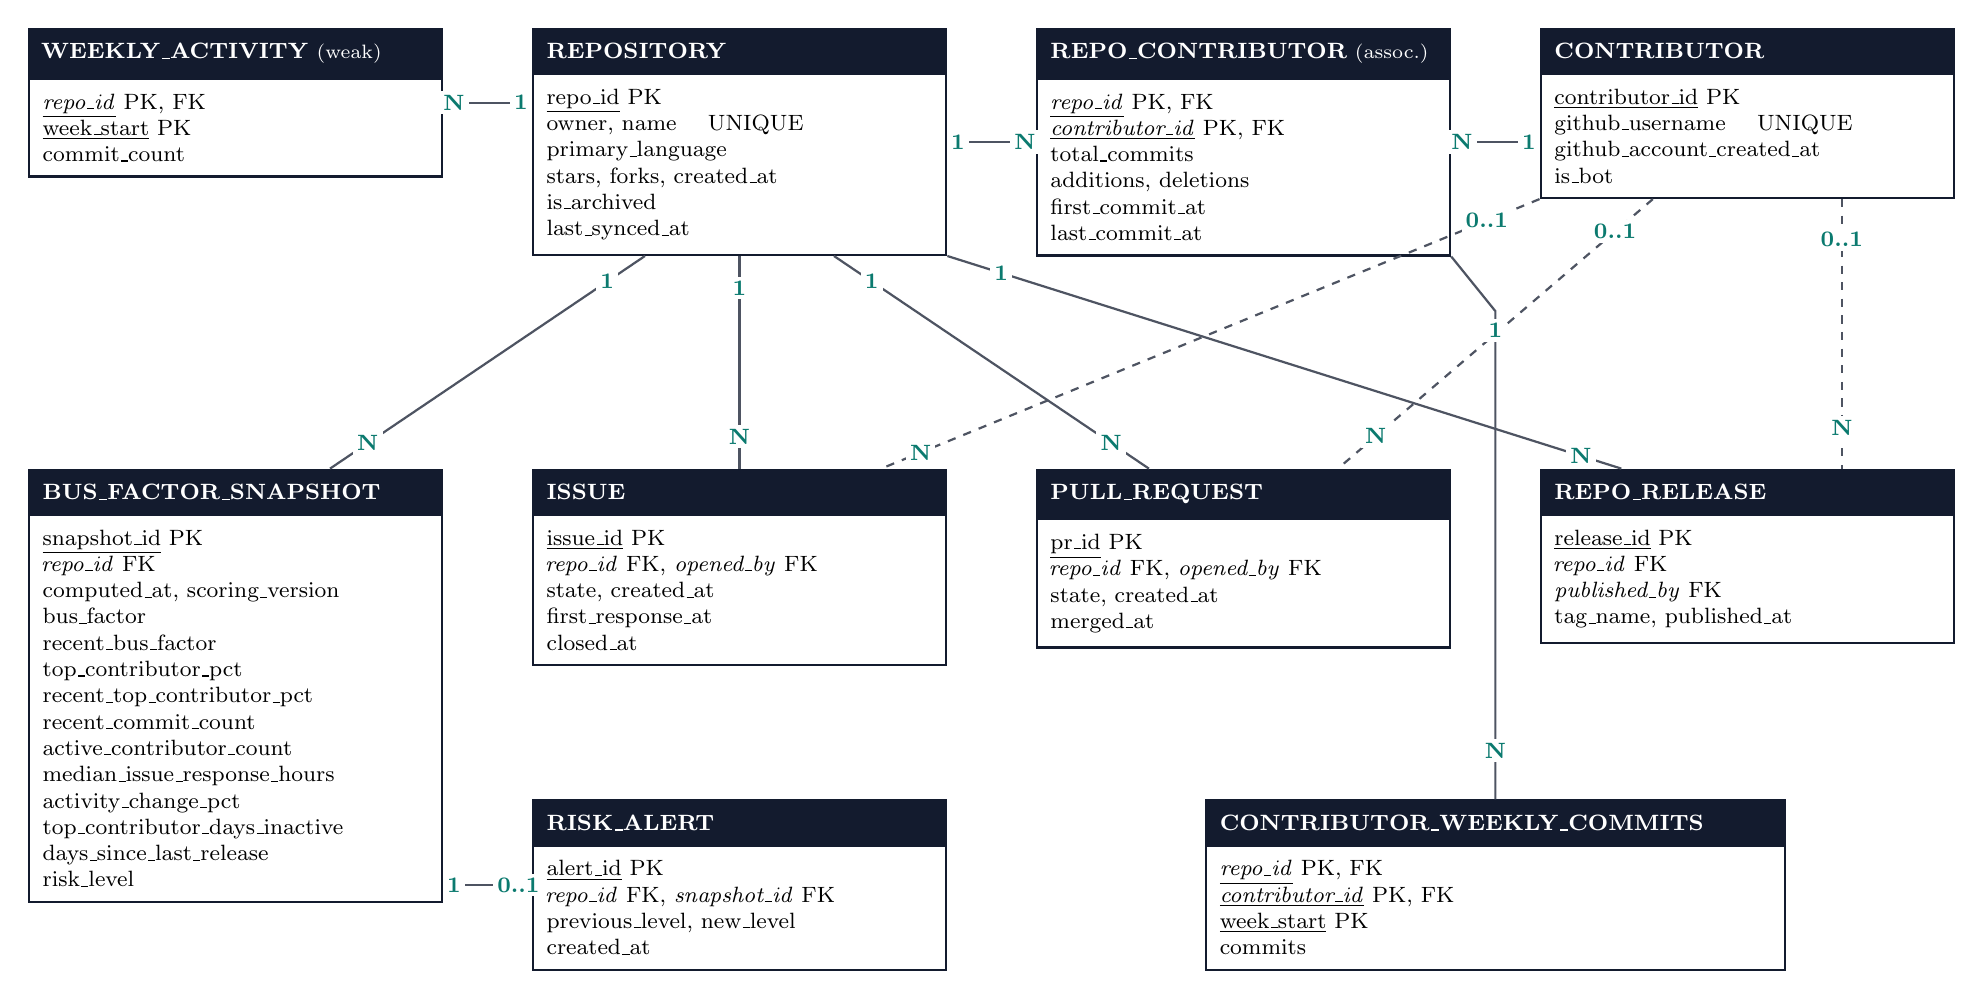
\begin{tikzpicture}[
  ent/.style={draw=navy, line width=0.8pt, rectangle split, rectangle split parts=2,
              rectangle split part fill={navy,white}, align=left, font=\footnotesize,
              inner sep=5pt, text width=4.9cm, anchor=north},
  rel/.style={line width=0.8pt, draw=navy!75},
  opt/.style={rel, dashed},
  card/.style={font=\footnotesize\bfseries, text=teal, fill=white, inner sep=1.5pt}
]
% Row 1
\node[ent] (wa) at (0,0) {\textcolor{white}{\textbf{WEEKLY\_ACTIVITY}} \textcolor{white}{\scriptsize(weak)}
  \nodepart{two} \underline{\textit{repo\_id}} PK, FK\\\underline{week\_start} PK\\commit\_count};
\node[ent] (repo) at (6.4,0) {\textcolor{white}{\textbf{REPOSITORY}}
  \nodepart{two} \underline{repo\_id} PK\\owner, name \quad UNIQUE\\primary\_language\\stars, forks, created\_at\\is\_archived\\last\_synced\_at};
\node[ent] (rc) at (12.8,0) {\textcolor{white}{\textbf{REPO\_CONTRIBUTOR}} \textcolor{white}{\scriptsize(assoc.)}
  \nodepart{two} \underline{\textit{repo\_id}} PK, FK\\\underline{\textit{contributor\_id}} PK, FK\\total\_commits\\additions, deletions\\first\_commit\_at\\last\_commit\_at};
\node[ent] (con) at (19.2,0) {\textcolor{white}{\textbf{CONTRIBUTOR}}
  \nodepart{two} \underline{contributor\_id} PK\\github\_username \quad UNIQUE\\github\_account\_created\_at\\is\_bot};
% Row 2
\node[ent] (snap) at (0,-5.6) {\textcolor{white}{\textbf{BUS\_FACTOR\_SNAPSHOT}}
  \nodepart{two} \underline{snapshot\_id} PK\\\textit{repo\_id} FK\\computed\_at, scoring\_version\\bus\_factor\\recent\_bus\_factor\\top\_contributor\_pct\\recent\_top\_contributor\_pct\\recent\_commit\_count\\active\_contributor\_count\\median\_issue\_response\_hours\\activity\_change\_pct\\top\_contributor\_days\_inactive\\days\_since\_last\_release\\risk\_level};
\node[ent] (iss) at (6.4,-5.6) {\textcolor{white}{\textbf{ISSUE}}
  \nodepart{two} \underline{issue\_id} PK\\\textit{repo\_id} FK, \textit{opened\_by} FK\\state, created\_at\\first\_response\_at\\closed\_at};
\node[ent] (pr) at (12.8,-5.6) {\textcolor{white}{\textbf{PULL\_REQUEST}}
  \nodepart{two} \underline{pr\_id} PK\\\textit{repo\_id} FK, \textit{opened\_by} FK\\state, created\_at\\merged\_at};
\node[ent] (rel) at (19.2,-5.6) {\textcolor{white}{\textbf{REPO\_RELEASE}}
  \nodepart{two} \underline{release\_id} PK\\\textit{repo\_id} FK\\\textit{published\_by} FK\\tag\_name, published\_at};
% Row 3
\node[ent] (alert) at (6.4,-9.8) {\textcolor{white}{\textbf{RISK\_ALERT}}
  \nodepart{two} \underline{alert\_id} PK\\\textit{repo\_id} FK, \textit{snapshot\_id} FK\\previous\_level, new\_level\\created\_at};
\node[ent, text width=7.0cm] (cwc) at (16.0,-9.8) {\textcolor{white}{\textbf{CONTRIBUTOR\_WEEKLY\_COMMITS}}
  \nodepart{two} \underline{\textit{repo\_id}} PK, FK\\\underline{\textit{contributor\_id}} PK, FK\\\underline{week\_start} PK\\commits};

% Repository relationships (1 : N)
\draw[rel] (repo.west |- wa.east) -- node[card, pos=0.12]{1} node[card, pos=0.88]{N} (wa.east);
\draw[rel] (repo.east |- rc.west) -- node[card, pos=0.12]{1} node[card, pos=0.88]{N} (rc.west);
\draw[rel] (repo.south) -- node[card, pos=0.15]{1} node[card, pos=0.85]{N} (iss.north);
\draw[rel] ([xshift=-1.2cm]repo.south) -- node[card, pos=0.12]{1} node[card, pos=0.88]{N} ([xshift=1.2cm]snap.north);
\draw[rel] ([xshift=1.2cm]repo.south) -- node[card, pos=0.12]{1} node[card, pos=0.88]{N} ([xshift=-1.2cm]pr.north);
\draw[rel] (repo.south east) -- node[card, pos=0.08]{1} node[card, pos=0.94]{N} ([xshift=-1.6cm]rel.north);
% Contributor relationships
\draw[rel] (con.west |- rc.east) -- node[card, pos=0.12]{1} node[card, pos=0.88]{N} (rc.east);
\draw[opt] ([xshift=1.2cm]con.south) -- node[card, pos=0.15]{0..1} node[card, pos=0.85]{N} ([xshift=1.2cm]rel.north);
\draw[opt] ([xshift=-1.2cm]con.south) -- node[card, pos=0.12]{0..1} node[card, pos=0.88]{N} ([xshift=1.2cm]pr.north);
\draw[opt] (con.south west) -- node[card, pos=0.08]{0..1} node[card, pos=0.94]{N} ([xshift=1.8cm]iss.north);
% Pair -> weeks
\draw[rel] (rc.south east) -- (16.0,-3.6) -- node[card, pos=0.04]{1} node[card, pos=0.9]{N} (cwc.north);
% Snapshot -> alert
\draw[rel] (snap.east |- alert.west) -- node[card, pos=0.12]{1} node[card, pos=0.85]{0..1} (alert.west);
\end{tikzpicture}}
\caption{Entity--relationship diagram. Underlined attributes form the primary key; italic
attributes are foreign keys. Solid lines are mandatory relationships, dashed lines optional
ones (a deleted GitHub account leaves the author unknown). \textsc{Contributor\_Weekly\_Commits}
breaks each repository--contributor pair down by week; its keys reference \textsc{Repository} and
\textsc{Contributor}. \textsc{Risk\_Alert} also references \textsc{Repository} (not drawn).}
\label{fig:er}
\end{figure}
\end{landscape}

\subsection{Relational schema}

The ER model maps to ten relations (Table~\ref{tab:schema}). GitHub's own
identifiers are used as primary keys for issues, pull requests and releases
(\texttt{BIGINT}), which makes re-syncing idempotent and guarantees that keys
never collide across repositories. \texttt{release} is a reserved word in
MySQL, hence \texttt{repo\_release}.

\begin{table}[H]
\centering
\caption{Relations, keys and purpose.}
\label{tab:schema}
\small
\begin{tabularx}{\textwidth}{>{\ttfamily}l >{\raggedright\arraybackslash}p{4.6cm} X}
\toprule
\textrm{\textbf{Relation}} & \textbf{Primary key / foreign keys} & \textbf{Purpose} \\
\midrule
repository & repo\_id; UNIQUE(owner, name) & One row per tracked repository \\
contributor & contributor\_id; UNIQUE(github\_username) & People and bots (\texttt{is\_bot}), shared across repositories \\
repo\_contributor & (repo\_id, contributor\_id) & Associative entity: commits per person per repository \\
contributor\_weekly\_commits & (repo\_id, contributor\_id, week\_start) & Weak entity: commits per person per week \\
issue & issue\_id; FK repo\_id, opened\_by & Issues with first-response time \\
pull\_request & pr\_id; FK repo\_id, opened\_by & Pull requests \\
repo\_release & release\_id; FK repo\_id, published\_by & Releases \\
weekly\_activity & (repo\_id, week\_start) & Weak entity: repository commits per week \\
bus\_factor\_snapshot & snapshot\_id; FK repo\_id & Append-only, versioned time series of computed risk \\
risk\_alert & alert\_id; FK repo\_id, snapshot\_id & Written by a trigger when risk increases \\
\bottomrule
\end{tabularx}
\end{table}

\paragraph{Referential integrity.} Every child relation references
\texttt{repository(repo\_id)} with \texttt{ON DELETE CASCADE}. Removing a
repository from the dashboard is therefore a single \texttt{DELETE} statement,
and the DBMS removes its contributor statistics, weekly commits, issues, pull
requests, releases, snapshots and alerts in the same operation. Contributors
are shared between repositories, so they are deliberately not cascaded.

\subsection{Normalisation}

All relations are in Boyce--Codd normal form: for every non-trivial functional
dependency $X \rightarrow Y$, $X$ is a superkey~\cite{codd1970relational,silberschatz2019db,elmasri2016fundamentals}.
Table~\ref{tab:nf} shows how each normal form is reflected in the design.

\begin{table}[H]
\centering
\caption{Normal forms as applied to the schema.}
\label{tab:nf}
\small
\begin{tabularx}{\textwidth}{l X}
\toprule
\textbf{Normal form} & \textbf{Application} \\
\midrule
1NF & Contributors of a repository are rows in \texttt{repo\_contributor}, not a
comma-separated list; weekly commits are one row per week, not an array. \\
2NF & In \texttt{contributor\_weekly\_commits}, \texttt{commits} depends on the
whole key (repository, contributor, week); \texttt{github\_username} and
\texttt{is\_bot} depend on \texttt{contributor\_id} alone and therefore live in
\texttt{contributor}. \\
3NF & \texttt{risk\_level} is derived from the bus factor and burnout signals and
changes on every sync, so it is stored on the snapshot that produced it, never
on \texttt{repository}. \\
BCNF & \texttt{repository} has two candidate keys, \texttt{repo\_id} and
(\texttt{owner}, \texttt{name}); both determine all other attributes. The same
holds for \texttt{contributor}. \\
\bottomrule
\end{tabularx}
\end{table}

\paragraph{Deliberate redundancy.} Two derived values are stored on purpose.
The \texttt{total\_commits} column of \texttt{repo\_contributor} is GitHub's
reported total for a contributor, kept so the contributor list can be read
without aggregating weekly rows. \texttt{bus\_factor\_snapshot} stores values that could in
principle be recomputed: a snapshot records what the measurements \emph{were}
at \texttt{computed\_at}, under the scoring method of that time.

\subsection{Indexes}

Besides primary keys and unique constraints, secondary indexes support the
most frequent access paths: \texttt{(repo\_id, week\_start)} on weekly commits
for windowed bus-factor queries, \texttt{(repo\_id, scoring\_version,
computed\_at)} on snapshots for ``latest snapshot'', trend and trigger
queries, \texttt{repo\_id} on \texttt{repo\_contributor} and \texttt{issue},
and \texttt{created\_at} on \texttt{risk\_alert} for the newest-first alert
feed.

\section{Transaction design}

Each repository is synchronised in one transaction (Listing~\ref{lst:txn}),
following the atomicity and durability guarantees of ACID
transactions~\cite{haerder1983principles}. If any step fails, such as a network error
during the preceding fetch, a malformed row or a lost database connection, the
whole repository rolls back. The previous snapshot then remains the latest
one, so the dashboard never shows a score computed from half-updated data.
Every write except the snapshots is an \texttt{INSERT \ldots\ ON DUPLICATE KEY
UPDATE}, making repeated syncs idempotent.

\begin{lstlisting}[language=Python, caption={Per-repository transaction (simplified from \texttt{sync\_repo}).}, label={lst:txn}]
cur = conn.cursor()            # conn.autocommit = False
try:
    repo_id = upsert_repo(cur, owner, repo, meta)
    for entry in contributor_stats:
        cid = upsert_contributor(cur, login, account_type)   # sets is_bot
        upsert_repo_contributor(cur, repo_id, cid, ...)
        upsert_contributor_weeks(cur, repo_id, cid, weeks)
    upsert_weekly_activity(cur, repo_id, commit_activity)
    for issue in issues:        upsert_issue(cur, repo_id, ...)
    for pr in pull_requests:    upsert_pull_request(cur, repo_id, ...)
    for release in releases:    upsert_release(cur, repo_id, ...)
    compute_and_insert_snapshot(cur, repo_id)   # back-fill if needed; fires the trigger
    conn.commit()
except Exception:
    conn.rollback()             # nothing for this repository is kept
    raise
\end{lstlisting}

\section{Computing the measurements in SQL}

All measurements are computed by one function, \texttt{compute\_metrics(repo,
as\_of)}, that takes the date the snapshot describes as a parameter. Today's
snapshot and the back-filled history (Section~\ref{sec:backfill}) are therefore
produced by exactly the same queries.

\subsection{Bus factor}

The bus factor of a time window is the smallest number of contributors who
together authored at least 50\% of the commits in that window, bots excluded.
Listing~\ref{lst:bf} computes it in a single pass: commits per person in the
window are summed from \texttt{contributor\_weekly\_commits}, people are ranked
by commits (ties broken by id so that the running total is strictly
cumulative), and the first rank at which the running total reaches half of
all commits is the bus factor.

\begin{lstlisting}[language=MySQL, caption={Bus factor over a window of weeks (after, until], bots excluded.}, label={lst:bf}]
WITH per_person AS (
    SELECT w.contributor_id, SUM(w.commits) AS commits
    FROM contributor_weekly_commits w
    JOIN contributor c ON c.contributor_id = w.contributor_id
    WHERE w.repo_id = %s AND c.is_bot = FALSE
      AND w.week_start > %s AND w.week_start <= %s
    GROUP BY w.contributor_id
),
ranked AS (
    SELECT contributor_id, commits,
           SUM(commits) OVER ()                                      AS total,
           SUM(commits) OVER (ORDER BY commits DESC, contributor_id) AS running_total,
           ROW_NUMBER() OVER (ORDER BY commits DESC, contributor_id) AS contributor_rank,
           COUNT(*)     OVER ()                                      AS people
    FROM per_person
)
SELECT MIN(CASE WHEN running_total >= 0.5 * total THEN contributor_rank END) AS bus_factor,
       MAX(CASE WHEN contributor_rank = 1
                THEN ROUND(100 * commits / total, 1) END)                   AS top_pct,
       MAX(total) AS commits, MAX(people) AS people
FROM ranked;
\end{lstlisting}

The query is run twice per snapshot:

\begin{itemize}
  \item \textbf{All-time:} every week up to the snapshot date.
  \item \textbf{Last 12 months:} the 52 weeks before the snapshot date.
\end{itemize}

The risk level is based on the \emph{recent} bus factor, which reflects who
maintains the project now, unless the repository had fewer than 10 non-bot
commits in those 12 months. In that case there is too little recent work to
measure, and the all-time value is used instead. The view exposes the value in
use as \texttt{effective\_bus\_factor}.

\subsection{Median issue-response time}

\texttt{PERCENTILE\_CONT} is only available from MySQL~8.0.28~\cite{mysql_manual}, so the
median uses a portable window-function form: response times of issues opened
in the 12 months before the snapshot date are numbered with
\texttt{ROW\_NUMBER()}, counted with \texttt{COUNT(*) OVER ()}, and the middle
one or two are averaged. At least five answered issues are required; otherwise
the median is reported as unknown.

\subsection{Burnout signals}

\begin{description}
  \item[No recent work.] Zero non-bot commits in the last 12 months.
  \item[Commit-activity change.] Non-bot commits per week in the most recent
        12 weeks compared with the 40 weeks before, computed by conditional
        aggregation over \texttt{contributor\_weekly\_commits}:
        \[
          \Delta_{\text{act}} = 100 \times
          \frac{\overline{c}_{\text{last 12 wk}} - \overline{c}_{\text{prev 40 wk}}}
               {\overline{c}_{\text{prev 40 wk}}} \;\%.
        \]
        Weeks without commits have no row, so sums are divided by the number
        of weeks (12 and 40) rather than averaged over rows. The change is only
        reported when the earlier period averaged at least one commit per week;
        below that a percentage is noise (one repository showed $+10{,}900\%$
        under the first version of the method).
  \item[Key-contributor inactivity.] Days since the last commit week of the
        top contributor in the window the rating is based on.
  \item[Slow issue response.] The median issue-response time described above.
\end{description}

Days since the latest release is also stored, but only as context: many
healthy libraries never publish GitHub releases.

\section{Risk scoring}

Algorithm~\ref{alg:risk} combines the measurements. The effective bus factor
sets a base level; an archived repository is Critical outright; and each
independent burnout signal raises the level by one, capped at Critical. The
function returns the level together with a list of plain-English reasons. The
same function is used by the sync engine (to store the level) and by the API
(to explain it), so the explanation always matches the stored score.

\begin{algorithm}[H]
\caption{Risk assessment (\texttt{assess\_risk})}
\label{alg:risk}
\begin{algorithmic}[1]
\Require all-time bus factor $b$, recent bus factor $b_r$ (or none), top-contributor share $s$ (\%)
         of the window in use, recent commits $n_r$, median response $m$ (h),
         activity change $a$ (\%), key-contributor inactivity $d$ (days), archived flag
\Ensure risk level $L \in \{0, 1, 2, 3\}$ (Healthy, Medium, High, Critical) and reasons $R$
\State $e \gets b_r$ \textbf{if} $b_r$ is defined \textbf{else} $b$
       \Comment{effective bus factor}
\State $L \gets 3$ \textbf{if} $e = 1$ \textbf{else} $2$ \textbf{if} $e = 2$
       \textbf{else} $1$ \textbf{if} $e \le 4$ \textbf{else} $0$
\State $R \gets$ [explanation of $e$, $s$ and, if different, $b$]
\If{archived} \State $L \gets 3$; add ``repository is archived'' to $R$ \EndIf
\If{$n_r = 0$} \State $L \gets L + 1$; add ``no commits in the last 12 months'' to $R$ \EndIf
\If{$m > 720$} \State $L \gets L + 1$; add ``slow issue responses'' to $R$ \EndIf
\If{$a \le -50$} \State $L \gets L + 1$; add ``commit activity down'' to $R$ \EndIf
\If{$d > 180$ \textbf{and} $s \ge 25$}
  \State $L \gets L + 1$; add ``top contributor inactive'' to $R$
\EndIf
\State \Return $(\min(L, 3),\ R)$
\end{algorithmic}
\end{algorithm}

\begin{table}[H]
\centering
\caption{Risk levels and burnout thresholds.}
\label{tab:thresholds}
\small
\begin{tabularx}{\textwidth}{l X l}
\toprule
\textbf{Component} & \textbf{Condition} & \textbf{Effect} \\
\midrule
Effective bus factor & 1 / 2 / 3--4 / $\ge 5$ & Critical / High / Medium / Healthy \\
Archived repository & \texttt{is\_archived = TRUE} & Critical \\
No recent work & no non-bot commits in the last 12 months & $+1$ level \\
Slow issue responses & median first human reply $> 30$ days ($\ge 5$ issues) & $+1$ level \\
Activity decline & last 12 weeks $\ge 50\%$ below previous 40 (baseline $\ge 1$/week) & $+1$ level \\
Key contributor inactive & no commit $> 180$ days \emph{and} share $\ge 25\%$ & $+1$ level \\
Release recency & days since last release & shown only \\
\bottomrule
\end{tabularx}
\end{table}

The 25\% share condition on the inactivity signal was added after testing on
real data (Section~\ref{sec:calibration}).

\section{History back-fill and scoring versions}
\label{sec:backfill}

\paragraph{Back-fill.} A daily sync only starts producing a trend after weeks
of snapshots. But \texttt{contributor\_weekly\_commits} holds each
contributor's commits since the repository began, so the past can be
measured directly. The first time a repository is scored with the current
method, \texttt{backfill\_history} calls \texttt{compute\_metrics} for the
first day of each of the previous 12 months, oldest first, and inserts one
snapshot per month with \texttt{computed\_at} set to that date. Issue
responses and releases are filtered to what was known at each date. Only the
archived flag cannot be reconstructed, since GitHub reports only its current
value, so back-filled snapshots treat the repository as active.

\paragraph{Scoring versions.} Changing how risk is computed creates a database
problem: comparing a snapshot from the old method with one from the new method
would report a change in the project that is really a change in the method.
Each snapshot therefore stores \texttt{scoring\_version} (1 = original
all-time method, 2 = bots excluded and recency-based). The view prefers the
newest version, and the procedure, the trigger, the trend endpoint and the
alerts feed only ever compare snapshots of the same version.

\section{Database objects}

\paragraph{View.} \texttt{v\_repo\_latest\_snapshot} joins every repository to
its newest snapshot (a \texttt{LEFT JOIN}, so repositories without a snapshot
still appear), ordering by \texttt{scoring\_version}, then
\texttt{computed\_at}, then \texttt{snapshot\_id}. Ordering by time rather
than insertion matters because the back-fill inserts past-dated rows. The view
also derives \texttt{effective\_bus\_factor} and
\texttt{effective\_top\_contributor\_pct} with \texttt{COALESCE}. All API
endpoints that need ``current state'' read from it.

\paragraph{Stored function.} \texttt{fn\_risk\_rank(level)} maps Healthy,
Medium, High and Critical to 1--4. The \texttt{ENUM} stores the levels in the
opposite order, so this function is the single definition of ``worse than'',
used by the trigger, the procedure and the API's risk ordering.

\paragraph{Stored procedure.} \texttt{sp\_declining\_repos(p\_days)} pairs each
repository's latest snapshot with the newest snapshot of the same scoring
version taken at least \texttt{p\_days} earlier, and returns repositories whose
effective bus factor fell or whose risk level rose.

\paragraph{Trigger.} \texttt{trg\_snapshot\_risk\_alert} (Listing~\ref{lst:trg})
fires after every snapshot insert. It compares the new risk level with the
repository's previous snapshot \emph{in time} and of the same scoring version,
and writes a row to \texttt{risk\_alert} when the risk has increased. The alert
is dated at the snapshot's own \texttt{computed\_at}, so alerts produced during
the back-fill carry the date the risk actually rose. Because the trigger runs
inside the sync transaction, a rolled-back sync can never leave an alert
pointing at a snapshot that does not exist.

\begin{lstlisting}[language=MySQL, caption={Trigger recording risk increases.}, label={lst:trg}]
CREATE TRIGGER trg_snapshot_risk_alert
AFTER INSERT ON bus_factor_snapshot
FOR EACH ROW
BEGIN
    DECLARE v_prev_level VARCHAR(10);
    SET v_prev_level = (
        SELECT s.risk_level FROM bus_factor_snapshot s
        WHERE s.repo_id = NEW.repo_id
          AND s.scoring_version = NEW.scoring_version
          AND s.snapshot_id <> NEW.snapshot_id
          AND s.computed_at < NEW.computed_at
        ORDER BY s.computed_at DESC, s.snapshot_id DESC
        LIMIT 1);
    IF v_prev_level IS NOT NULL
       AND fn_risk_rank(NEW.risk_level) > fn_risk_rank(v_prev_level) THEN
        INSERT INTO risk_alert (repo_id, snapshot_id, previous_level, new_level, created_at)
        VALUES (NEW.repo_id, NEW.snapshot_id, v_prev_level, NEW.risk_level, NEW.computed_at);
    END IF;
END
\end{lstlisting}

\section{Application layer}

\paragraph{REST API.} A FastAPI~\cite{fastapi} service exposes nine endpoints:
a risk-ranked repository list with filtering and sorting, repository detail
with contributor breakdown (bots marked, last-12-months commits) and risk
reasons, snapshot history, dashboard summary counts, declining repositories
(via the stored procedure), recent alerts, GitHub search, and adding or
removing a tracked repository. The trend endpoint keeps one point per day,
the day's latest snapshot, using \texttt{ROW\_NUMBER()} partitioned by date.
Database connections come from a pool of five; every query is parameterised.

\paragraph{Dashboard.} A React~\cite{react} single-page application
(Figure~\ref{fig:dashboard}) shows summary counts per risk level, the recent
risk increases, and a searchable, filterable risk-ranked table. The detail page
(Figures~\ref{fig:detail} and~\ref{fig:trend}) shows both bus factors, the
reasons for the risk level, the burnout signals, the bus-factor trend and the
contributor breakdown.

% ===========================================================================
\chapter{Results and Discussion}
\label{ch:results}
% ===========================================================================

\section{Experimental setup}

The system was run on a Windows~11 laptop with MySQL Community Server 8.0.46,
Python~3.12 and Node.js. The tracked list contained 43 public repositories:
large, well-staffed projects (e.g.\ React, Kubernetes, CPython, Rust),
popular single-maintainer utilities (e.g.\ \texttt{is-number}, \texttt{p-limit},
\texttt{chalk}), libraries known to be in maintenance mode or deprecated
(\texttt{request}, \texttt{moment}) and one archived project
(\texttt{jquery-mobile}). All figures below use each repository's latest
snapshot (scoring version~2) from the sync of 17 October 2026, and the 12
monthly snapshots back-filled from November 2025 to October 2026.

\section{Data collected}

One repository (\texttt{substack/node-mkdirp}) no longer exists on GitHub and
returned HTTP 404; the remaining 42 were synchronised. Table~\ref{tab:counts}
lists the resulting row counts; the database occupies 44\,MB including
indexes.

\begin{table}[H]
\centering
\caption{Rows stored per relation.}
\label{tab:counts}
\small
\begin{tabular}{lr@{\hspace{3em}}lr}
\toprule
\textbf{Relation} & \textbf{Rows} & \textbf{Relation} & \textbf{Rows} \\
\midrule
repository & 42 & pull\_request & 16,490 \\
contributor (52 bots) & 17,306 & repo\_release & 3,145 \\
repo\_contributor & 10,053 & weekly\_activity & 2,549 \\
contributor\_weekly\_commits & 273,603 & bus\_factor\_snapshot & 833 \\
issue & 6,211 & risk\_alert & 25 \\
\bottomrule
\end{tabular}
\end{table}

Of the 833 snapshots, 631 were produced by scoring version~2 (547 of them by the
back-fill); 16 of the 25 alerts belong to version~2.

\paragraph{Correcting the response times.} The first version of the sync took
the very first comment on an issue as its response. When the bot-aware rule was
introduced, a maintenance script re-fetched the 1,043 stored response times
that could still be looked up. 217 changed, including 89 issues whose only
comments came from bots or the issue's author. The 467 that could no longer be
looked up were cleared rather than kept, leaving 954 verified response times.

\section{Risk distribution}

Figure~\ref{fig:dist} and Table~\ref{tab:dist} summarise the risk levels.
\textbf{21 of the 42 repositories (50\%) have an effective bus factor of~1}:
one person wrote at least half of their recent commits (or, for the seven
repositories with fewer than 10 recent commits, of all commits). After the
burnout signals are applied, 27 repositories are Critical, 2 High, 2 Medium and
11 Healthy.

\begin{figure}[H]
\centering
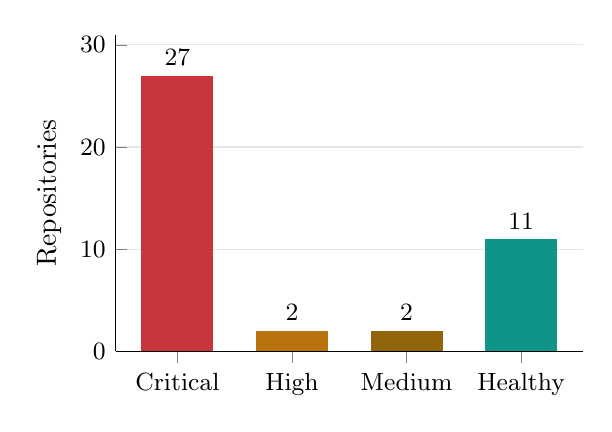
\begin{tikzpicture}
\begin{axis}[
  ybar, bar width=26pt, bar shift=0pt, width=0.62\textwidth, height=5.6cm,
  symbolic x coords={Critical,High,Medium,Healthy}, xtick={Critical,High,Medium,Healthy},
  ymin=0, ymax=31, ylabel={Repositories},
  nodes near coords, nodes near coords style={font=\small},
  axis lines*=left, ymajorgrids, grid style={gray!20},
  enlarge x limits=0.18, tick label style={font=\small}
]
\addplot[fill=crit, draw=none] coordinates {(Critical,27)};
\addplot[fill=high, draw=none] coordinates {(High,2)};
\addplot[fill=med, draw=none] coordinates {(Medium,2)};
\addplot[fill=healthy, draw=none] coordinates {(Healthy,11)};
\end{axis}
\end{tikzpicture}
\caption{Risk level of the 42 repositories (latest snapshot).}
\label{fig:dist}
\end{figure}

\begin{table}[H]
\centering
\caption{Risk levels with average effective bus factor and top-contributor share.}
\label{tab:dist}
\small
\begin{tabular}{lrrr}
\toprule
\textbf{Risk level} & \textbf{Repositories} & \textbf{Avg.\ bus factor} & \textbf{Avg.\ top-contributor share} \\
\midrule
Critical & 27 & 1.3 & 70.4\% \\
High & 2 & 2.0 & 44.7\% \\
Medium & 2 & 4.0 & 24.5\% \\
Healthy & 11 & 12.4 & 10.7\% \\
\bottomrule
\end{tabular}
\end{table}

Figure~\ref{fig:scatter} plots each repository's effective bus factor against
its top contributor's share of commits in the same window. Every repository
whose top contributor wrote more than half of the commits has a bus factor of~1
by definition, and every Healthy repository has a top contributor below 25\%.
Popularity offers no protection: \texttt{scrcpy} (over 150,000 stars) has a
bus factor of~1, with 89.7\% of last year's commits from one person, and
\texttt{flask} (75,000 stars) has 96.2\%.

\begin{figure}[H]
\centering
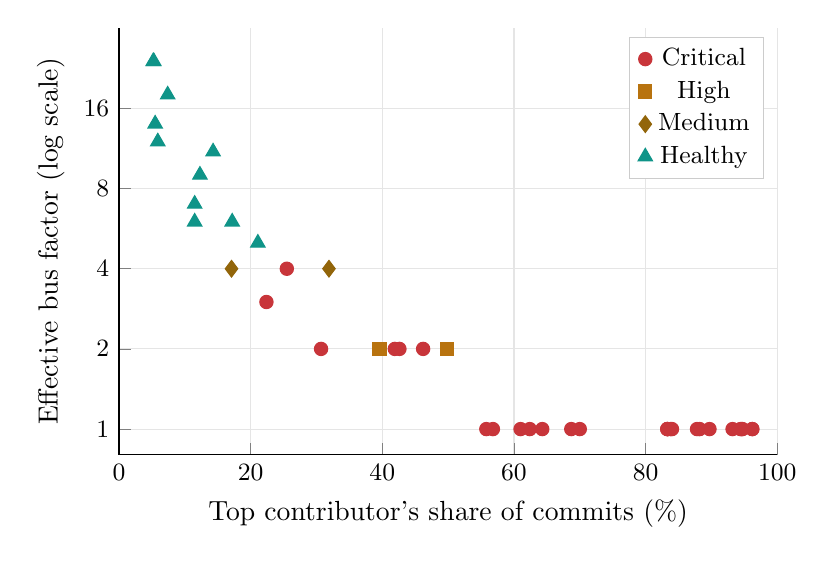
\begin{tikzpicture}
\begin{axis}[
  width=0.82\textwidth, height=7cm,
  xlabel={Top contributor's share of commits (\%)},
  ylabel={Effective bus factor (log scale)},
  ymode=log, log basis y=2, ymin=0.8, ymax=32,
  ytick={1,2,4,8,16}, yticklabels={1,2,4,8,16},
  xmin=0, xmax=100, axis lines*=left, grid=major, grid style={gray!20},
  legend style={at={(0.98,0.98)}, anchor=north east, font=\small, draw=gray!40},
  tick label style={font=\small}
]
\addplot[only marks, mark=*, mark size=2.4pt, color=crit] coordinates {
 (89.7,1) (61.0,1) (96.2,1) (64.3,1) (62.4,1) (94.7,1) (87.8,1) (84.0,1)
 (70.0,1) (83.8,1) (83.3,1) (88.2,1) (93.2,1) (56.8,1) (83.3,1) (94.4,1)
 (68.7,1) (94.6,1) (83.3,1) (55.8,1) (96.2,1) (42.6,2) (41.9,2) (30.7,2)
 (46.2,2) (22.4,3) (25.5,4)};
\addplot[only marks, mark=square*, mark size=2.4pt, color=high] coordinates {
 (39.6,2) (49.8,2)};
\addplot[only marks, mark=diamond*, mark size=3pt, color=med] coordinates {
 (31.9,4) (17.1,4)};
\addplot[only marks, mark=triangle*, mark size=3pt, color=healthy] coordinates {
 (21.1,5) (11.5,6) (17.2,6) (11.5,7) (12.3,9) (14.3,11) (5.9,12) (5.5,14)
 (7.4,18) (5.3,24) (5.2,24)};
\legend{Critical, High, Medium, Healthy}
\end{axis}
\end{tikzpicture}
\caption{Effective bus factor versus top-contributor share for the 42 repositories.}
\label{fig:scatter}
\end{figure}

Concentration is also uneven across ecosystems (Table~\ref{tab:lang}). The 20
JavaScript repositories have an average effective bus factor of 2.0, against
5.4 for the 8 Python repositories, which reflects the many small
single-purpose npm packages in the sample. The sample per language is small and
was not drawn randomly, so this is an observation about this data set, not a
general claim.

\begin{table}[H]
\centering
\caption{Average effective bus factor by primary language (languages with $\ge 2$ repositories).}
\label{tab:lang}
\small
\begin{tabular}{lrr}
\toprule
\textbf{Language} & \textbf{Repositories} & \textbf{Avg.\ bus factor} \\
\midrule
JavaScript & 20 & 2.0 \\
Python & 8 & 5.4 \\
TypeScript & 5 & 4.2 \\
Go & 2 & 16.0 \\
C & 2 & 2.5 \\
\bottomrule
\end{tabular}
\end{table}

\section{Effect of excluding bots and measuring recent work}

\paragraph{Bots.} Excluding the 52 bot accounts changes large projects most.
Kubernetes' all-time bus factor rises from 18 to 44 once
\nolinkurl{k8s-ci-robot} (27,260 commits) is excluded, and TensorFlow's from 18
to 76 without \nolinkurl{tensorflower-gardener} (59,810 commits). Both are
Healthy either way, but their reported top contributor is now a person.

\paragraph{Recency.} For 35 of the 42 repositories the rating is based on the
last 12 months; the other seven had fewer than 10 recent commits. Measuring
recent work corrects cases in both directions:

\begin{itemize}
  \item \textbf{Express} has an all-time bus factor of~1 (its original author
        wrote most of its history) but a recent bus factor of~2: it is rated
        High, not Critical.
  \item \textbf{Flask} goes the other way: its all-time bus factor is 2, but one
        maintainer wrote 96.2\% of last year's commits, a recent bus factor of~1.
  \item \textbf{jQuery} (all-time 4, recent 1) and \textbf{requests} (all-time
        3, recent 1) likewise now depend on a single active maintainer.
\end{itemize}

\paragraph{Burnout signals.} Across the 42 repositories, the key-contributor
inactivity signal fired for 6, a commit-activity fall of 50\% or more for 4,
and ``no commits in the last 12 months'' for 4 (\texttt{is-number},
\texttt{request}, \texttt{jquery-mobile}, \texttt{gulp}). One repository is
archived. With bot replies removed, no repository's median issue response
exceeded 30 days.

\section{Trends and alerts}

The back-filled history makes the trend features usable immediately. The call
\begin{center}
\texttt{CALL sp\_declining\_repos(180);}
\end{center}
returns 12 repositories whose effective bus factor fell or whose risk rose over
the last six months. The clearest case,
\texttt{httpx}, is shown in Figure~\ref{fig:trend}: its bus factor was between
4 and 5 from December 2025 to August 2026, and has been 1 since September. Recent activity fell below
10 commits a year, so the rating now rests on the all-time bus factor, which is
dominated by its original author, who has not committed for 398 days.

\begin{figure}[H]
\centering
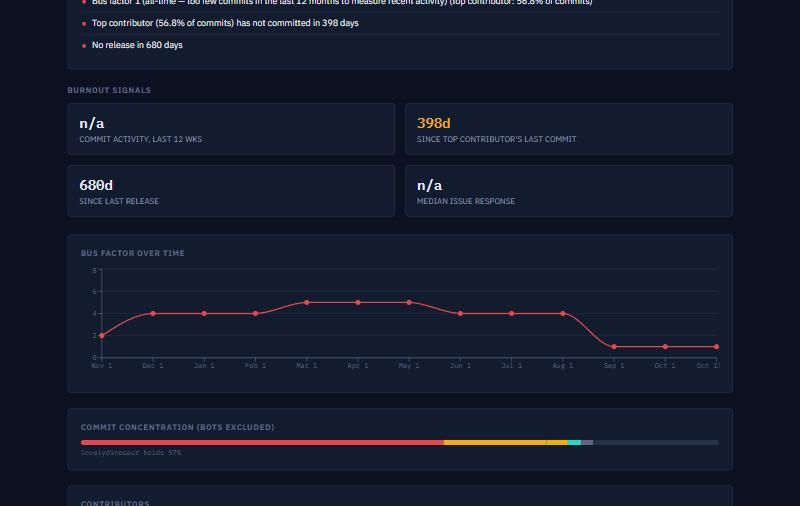
\includegraphics[width=0.92\textwidth]{figures/trend.jpg}
\caption{Bus factor over time for \texttt{encode/httpx}: monthly back-filled
snapshots from November 2025 and the current one.}
\label{fig:trend}
\end{figure}

The trigger recorded 16 risk increases in the version-2 history
(Table~\ref{tab:alerts}), each dated at the snapshot where the risk rose.

\begin{table}[H]
\centering
\caption{Risk increases recorded by \texttt{trg\_snapshot\_risk\_alert} (scoring version~2).}
\label{tab:alerts}
\small
\begin{tabular}{llll}
\toprule
\textbf{Date} & \textbf{Repository} & \textbf{Before} & \textbf{After} \\
\midrule
2025-12-01 & gulpjs/gulp & Medium & High \\
2026-01-01 & psf/requests & High & Critical \\
2026-02-01 & facebook/react & Medium & High \\
2026-03-01 & jashkenas/underscore & High & Critical \\
2026-03-01 & expressjs/express & Medium & High \\
2026-04-01 & encode/httpx & Healthy & Medium \\
2026-05-01 & facebook/react & Medium & High \\
2026-05-01 & expressjs/express & High & Critical \\
2026-06-01 & gulpjs/gulp & High & Critical \\
2026-06-01 & encode/httpx & Medium & High \\
2026-07-01 & django/django & Healthy & Medium \\
2026-07-01 & sindresorhus/execa & High & Critical \\
2026-09-01 & encode/httpx & High & Critical \\
2026-10-01 & lodash/lodash & High & Critical \\
2026-10-17 & pypa/pip & High & Critical \\
2026-10-17 & jquery/jquery-mobile & High & Critical \\
\bottomrule
\end{tabular}
\end{table}

Two caveats apply. Alerts that were followed by a recovery remain in the log,
which is intended: React rose to High twice and is Healthy today. And
\texttt{jquery-mobile}'s alert on 17 October reflects the archived flag, which
is only known for today, not a change on that day.

\section{Case studies and validation}
\label{sec:calibration}

Figure~\ref{fig:detail} shows the explanation produced for \texttt{httpx}.
Several cases act as sanity checks on the method:

\begin{itemize}
  \item \textbf{Known-healthy projects score Healthy.} React, Node.js, Rust,
        PyTorch, CPython, Kubernetes, Go and VS Code all have effective bus
        factors of 5 or more, with no contributor above 22\% of recent commits.
  \item \textbf{Known-unmaintained projects score badly.} The archived
        \texttt{jquery-mobile}, the deprecated \texttt{request} and the
        maintenance-mode \texttt{moment} are all Critical.
  \item \textbf{Calibration of the inactivity signal.} In a first version the
        inactivity signal fired whenever the top contributor had been silent
        for 180 days. This rated React as Medium because its all-time top
        contributor, with only 10.2\% of commits, had not committed for 264
        days. Such turnover is routine in a large project, so the signal now
        requires the inactive person to hold at least 25\% of commits.
\end{itemize}

\begin{figure}[H]
\centering
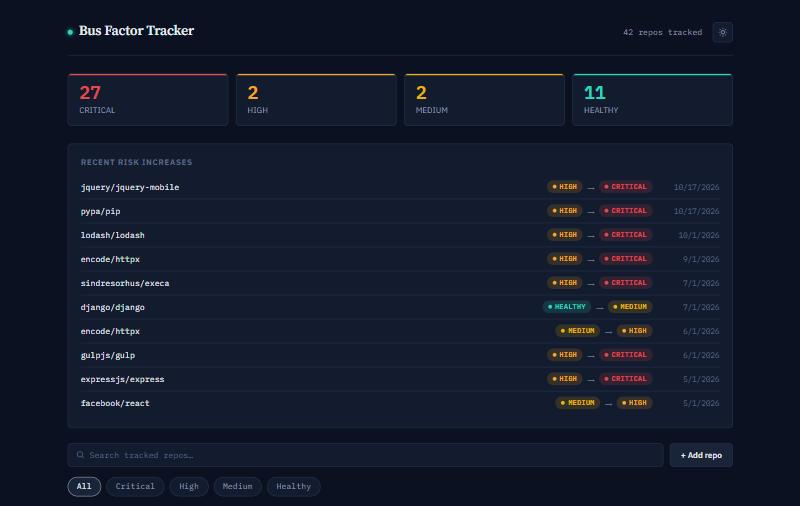
\includegraphics[width=0.92\textwidth]{figures/dashboard.jpg}
\caption{Dashboard: summary counts per risk level and the recent risk
increases recorded by the trigger, dated by when the risk rose.}
\label{fig:dashboard}
\end{figure}

\begin{figure}[H]
\centering
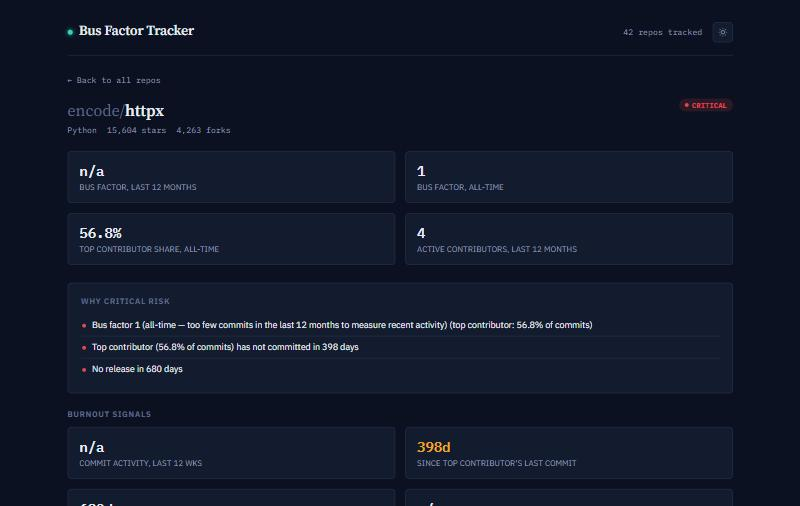
\includegraphics[width=0.92\textwidth]{figures/repo_detail.jpg}
\caption{Repository detail for \texttt{encode/httpx}: recent and all-time bus
factor, the reasons for the risk level, and the burnout signals.}
\label{fig:detail}
\end{figure}

\section{Performance}

\paragraph{Sync.} The full sync of 43 repositories with scoring version~2
took 1,267.9\,s (about 29\,s per repository). It wrote 273,603 weekly commit
rows and back-filled 547 snapshots, and the time is dominated by GitHub API
latency. During the run the engine recovered from repeated dropped and
truncated connections without losing any repository.

\paragraph{API.} Table~\ref{tab:latency} shows the median latency of each read
endpoint over 20 requests, measured in-process against the local database.
The repository-detail endpoint originally took 186\,ms for React because its
commit-share column used a correlated subquery that re-summed the repository's
commits for every one of its 504 contributor rows. Replacing it with the
window function \texttt{SUM(\ldots) OVER ()} computes the total once. Even with
the per-contributor last-12-months join added later, the endpoint takes
10.4\,ms.

\begin{table}[H]
\centering
\caption{Median API latency over 20 requests.}
\label{tab:latency}
\small
\begin{tabular}{lr}
\toprule
\textbf{Endpoint} & \textbf{Median latency} \\
\midrule
\texttt{GET /api/repos} (risk-ranked list, via view) & 6.0\,ms \\
\texttt{GET /api/repos/facebook/react} (correlated subquery, v1) & 186.3\,ms \\
\texttt{GET /api/repos/facebook/react} (window function) & 10.4\,ms \\
\texttt{GET /api/repos/\{owner\}/\{name\}/trend} & 4.0\,ms \\
\texttt{GET /api/stats/summary} & 4.9\,ms \\
\texttt{GET /api/stats/declining} (stored procedure) & 6.6\,ms \\
\texttt{GET /api/alerts} & 4.0\,ms \\
\bottomrule
\end{tabular}
\end{table}

\section{Per-repository results}

Table~\ref{tab:all} lists the latest snapshot for every repository.

\begin{small}
\setlength{\tabcolsep}{4pt}
\begin{longtable}{l l r r r r r l}
\caption{Latest snapshot per repository (bots excluded). BF 12m = bus factor
over the last 12 months (``--'' = fewer than 10 recent commits); BF all =
all-time bus factor; Top = top contributor's share of commits in the window
the rating uses; $\Delta$Act = commit-activity change (``--'' = baseline below
one commit per week); Inact.\ = days since that contributor's last commit.}
\label{tab:all}\\
\toprule
\textbf{Repository} & \textbf{Lang.} & \textbf{BF 12m} & \textbf{BF all} & \textbf{Top \%} & \textbf{$\Delta$Act \%} & \textbf{Inact.} & \textbf{Risk} \\
\midrule
\endfirsthead
\toprule
\textbf{Repository} & \textbf{Lang.} & \textbf{BF 12m} & \textbf{BF all} & \textbf{Top \%} & \textbf{$\Delta$Act \%} & \textbf{Inact.} & \textbf{Risk} \\
\midrule
\endhead
\bottomrule
\endfoot
Genymobile/scrcpy & C & 1 & 1 & 89.7 & 7.3 & 13 & \risk{Critical} \\
laravel/laravel & Blade & 1 & 1 & 61.0 & $-61.4$ & 13 & \risk{Critical} \\
pallets/flask & Python & 1 & 2 & 96.2 & 8.3 & 13 & \risk{Critical} \\
jquery/jquery & JS & 1 & 4 & 64.3 & $-27.5$ & 13 & \risk{Critical} \\
vuejs/core & TS & 1 & 1 & 62.4 & $-12.4$ & 6 & \risk{Critical} \\
psf/requests & Python & 1 & 3 & 94.7 & $-94.0$ & 55 & \risk{Critical} \\
moment/moment & JS & 1 & 2 & 87.8 & -- & 34 & \risk{Critical} \\
tj/commander.js & JS & 1 & 1 & 84.0 & -- & 146 & \risk{Critical} \\
Automattic/mongoose & JS & 1 & 1 & 70.0 & $-20.5$ & 6 & \risk{Critical} \\
jashkenas/underscore & JS & 1 & 3 & 83.8 & -- & 6 & \risk{Critical} \\
chalk/chalk & JS & 1 & 1 & 83.3 & -- & 20 & \risk{Critical} \\
motdotla/dotenv & JS & 1 & 1 & 88.2 & 78.7 & 6 & \risk{Critical} \\
sindresorhus/ky & TS & 1 & 1 & 93.2 & 290.2 & 13 & \risk{Critical} \\
BtbN/FFmpeg-Builds & Shell & 1 & 1 & 83.3 & 145.2 & 20 & \risk{Critical} \\
benoitc/gunicorn & Python & 1 & 1 & 94.4 & $-1.3$ & 41 & \risk{Critical} \\
cordiverse/cordis & TS & 1 & 1 & 68.7 & 386.3 & 6 & \risk{Critical} \\
sindresorhus/execa & JS & 1 & 1 & 94.6 & -- & 6 & \risk{Critical} \\
sindresorhus/p-limit & JS & 1 & 1 & 83.3 & -- & 34 & \risk{Critical} \\
encode/httpx & Python & -- & 1 & 56.8 & -- & 398 & \risk{Critical} \\
sindresorhus/is-online & JS & -- & 1 & 55.8 & -- & 34 & \risk{Critical} \\
jonschlinkert/is-number & JS & -- & 1 & 96.2 & -- & 3,030 & \risk{Critical} \\
lodash/lodash & JS & 2 & 1 & 42.6 & $-85.2$ & 181 & \risk{Critical} \\
pypa/pip & Python & 2 & 6 & 46.2 & $-51.4$ & 6 & \risk{Critical} \\
caolan/async & JS & -- & 2 & 41.9 & -- & 776 & \risk{Critical} \\
request/request & JS & -- & 2 & 30.7 & -- & 2,442 & \risk{Critical} \\
jquery/jquery-mobile$^{\dagger}$ & JS & -- & 3 & 22.4 & -- & 3,702 & \risk{Critical} \\
gulpjs/gulp & JS & -- & 4 & 25.5 & -- & 503 & \risk{Critical} \\
expressjs/express & JS & 2 & 1 & 39.6 & -- & 97 & \risk{High} \\
mochajs/mocha & JS & 2 & 3 & 49.8 & 0.7 & 13 & \risk{High} \\
django/django & Python & 4 & 8 & 31.9 & $-31.9$ & 6 & \risk{Medium} \\
FFmpeg/FFmpeg & C & 4 & 5 & 17.1 & 20.5 & 48 & \risk{Medium} \\
facebook/react & JS & 5 & 6 & 21.1 & $-17.6$ & 6 & \risk{Healthy} \\
angular/angular & TS & 6 & 14 & 11.5 & $-22.1$ & 6 & \risk{Healthy} \\
rails/rails & Ruby & 6 & 13 & 17.2 & 39.7 & 6 & \risk{Healthy} \\
nodejs/node & JS & 7 & 13 & 11.5 & 117.0 & 6 & \risk{Healthy} \\
python/cpython & Python & 9 & 14 & 12.3 & $-1.2$ & 6 & \risk{Healthy} \\
rust-lang/rust & Rust & 11 & 20 & 14.3 & 17.9 & 6 & \risk{Healthy} \\
microsoft/vscode & TS & 12 & 7 & 5.9 & $-8.6$ & 6 & \risk{Healthy} \\
golang/go & Go & 14 & 12 & 5.5 & 15.3 & 13 & \risk{Healthy} \\
kubernetes/kubernetes & Go & 18 & 44 & 7.4 & $-41.0$ & 6 & \risk{Healthy} \\
tensorflow/tensorflow & C++ & 24 & 76 & 5.3 & 9.8 & 13 & \risk{Healthy} \\
pytorch/pytorch & Python & 24 & 49 & 5.2 & 9.1 & 6 & \risk{Healthy} \\
\end{longtable}
\end{small}
\vspace{-1em}
\noindent{\footnotesize $^{\dagger}$Archived by its owner.}

\section{Discussion of limitations}

The second version of the method removes the three main weaknesses found in
the first: bots counted as contributors, an all-time bus factor that
over-weighted people who left long ago, and the absence of history before the
first sync. The following limitations remain:

\begin{itemize}
  \item \textbf{Commits are a proxy for effort.} Code review, issue triage,
        releases and documentation are not counted, and in projects where
        committers apply other people's patches (as in Django) commits credit
        the person who merges.
  \item \textbf{Bot detection is name-based.} A bot with an ordinary-looking
        name is not caught. Go's median issue response is still under an hour,
        which may come from such an account.
  \item \textbf{Contributor statistics are capped.} GitHub's statistics cover
        each repository's top 100 contributors, so the long tail of very large
        projects is incomplete. Commits from e-mail addresses not linked to a
        GitHub account are missing altogether.
  \item \textbf{Switching to the all-time bus factor can cause a jump.} When a
        repository's recent activity falls below 10 commits a year, the rating
        moves from the recent to the all-time bus factor, as for \texttt{httpx}
        in September 2026. The reasons list states this explicitly.
  \item \textbf{Some history cannot be reconstructed.} The archived flag is
        only known for today, and response times are sparse for older issues,
        so back-filled snapshots rely mainly on commit data.
  \item \textbf{The sample is small and hand-picked.} 42 repositories chosen to
        cover healthy, small and abandoned projects are enough to test the
        method, not to draw ecosystem-wide conclusions.
\end{itemize}

\section{Challenges and lessons learned}

\begin{itemize}
  \item \textbf{A query that silently returned nothing.} The first trend query
        joined snapshots on \texttt{s2.computed\_at = s1.computed\_at - INTERVAL
        6 MONTH}. Snapshots are taken whenever the sync runs, so no two are
        exactly six months apart to the second, and the query always returned
        zero rows. It now selects the newest snapshot \emph{at or before} the
        cut-off. Lesson: test every query on real data, not just for syntax.
  \item \textbf{Bots in the data.} Real data showed CI bots ranked as the top
        contributors of Kubernetes, TensorFlow and PyTorch, and bots replying to
        every new issue within seconds. Both distort the measurements and are
        now filtered out.
  \item \textbf{Changing the method without corrupting the history.} The first
        re-score under the new method would have looked like a wave of real
        risk changes. Versioned snapshots, compared only within a version,
        keep method changes and project changes apart.
  \item \textbf{Driver behaviour.} The installed MySQL connector returns
        stored-procedure results as dictionaries, which broke the API's
        tuple-based handling only once real rows existed. The endpoint now
        accepts both forms.
  \item \textbf{Porting from PostgreSQL to MySQL.} The design was first written
        for PostgreSQL. MySQL needed a different \texttt{INTERVAL} syntax, a
        window-function median instead of \texttt{PERCENTILE\_CONT}, and a
        renamed \texttt{release} table.
  \item \textbf{Calibrating on real data.} The React case showed that a signal
        that looks reasonable in isolation can mislabel large projects;
        thresholds must be checked against known cases.
\end{itemize}

% ===========================================================================
\chapter{Conclusion and Future Work}
\label{ch:conclusion}
% ===========================================================================

\section{Conclusion}

This project built a working, database-centred system that estimates the bus
factor and maintainer-burnout risk of real open-source repositories using only
public GitHub data. The design applies core DBMS concepts where they solve real
problems:
\begin{itemize}
  \item a normalised schema in BCNF with cascading referential integrity;
  \item one ACID transaction per repository, so a failed sync never corrupts
        the current state;
  \item CTEs and window functions that compute every measurement inside the
        database, for any time window and as of any past date;
  \item a view, stored function, stored procedure and trigger that expose
        current risk, detect declines and record risk increases;
  \item versioned snapshots, so the method can change without corrupting the
        history.
\end{itemize}

On 42 widely used repositories the system showed that the risk is
widespread: half of them depend on one person for at least half of their
recent commits, including projects with tens of thousands of stars. A year of
history rebuilt from weekly commit data revealed 16 risk increases and declines
such as \texttt{httpx}'s fall from a bus factor of 5 to~1. Every risk level is
explained in plain English, and the API answers in about 10\,ms.

\section{Future work}

\begin{itemize}
  \item Count review, triage and release work, not only commits.
  \item Read commit history from cloned repositories to include contributors
        beyond GitHub's top 100 and commits from unlinked e-mail addresses.
  \item Analyse a project's full dependency tree to report the riskiest
        dependencies of an application.
  \item Send e-mail or webhook notifications when a tracked repository becomes
        Critical.
  \item Validate the risk levels against a labelled set of projects that were
        later abandoned.
\end{itemize}

% ---------------------------------------------------------------------------
\cleardoublepage
\phantomsection
\addcontentsline{toc}{chapter}{References}
\bibliographystyle{unsrtnat}
\bibliography{references}

\end{document}
